\documentclass{article}

\usepackage{amsmath} % Define various maths environments
\usepackage{amssymb} % Define various maths symbols
\usepackage{geometry} % Adjust the margin, paper size, and etc.
\geometry{a4paper, scale = 0.8}
\usepackage{enumerate} % Provide different style of lists
\usepackage{graphicx} % Insert image of all types
\usepackage{xcolor}
\usepackage{ulem}
\usepackage{pdfpages}
\usepackage{array} % Provide auxiliary farmat for tabular
\usepackage{booktabs} % Create Three-line Table
\usepackage{bm}
\usepackage{cite}
\usepackage{url}
\usepackage{float}
\usepackage{indentfirst}
\usepackage{multirow}
\usepackage[colorlinks,linkcolor=black]{hyperref}
\usepackage{subfigure}

\begin{document}

\vspace*{0.4cm}

\hrulefill %??????draw a horizontal line??????

\thispagestyle{empty} %set empty in footnote

\begin{center}
\begin{large}
\scshape{UM--SJTU Joint Institute \vspace{0.3em} \\ Physics Laboratory \\(Vp241)}
\end{large}

\hrulefill %??????draw a horizontal line??????

\vspace*{7.5cm}
\begin{Large}
\scshape{{Laboratory Report}}
\end{Large}

\vspace{2.5em}

\begin{large}
\scshape{Exercise 2}\\
\vspace{0.5em}
\scshape{The Hall Probe: Characteristics and Applications}
\end{large}
\end{center}

\vspace{13em}

\begin{table}[h!]
\center
\begin{tabular}{lll}
Name: Haoming  Zhu \hspace*{2em}&
ID: 520021910145\hspace*{2em}
& Group: 1 \\
\end{tabular}
\end{table}

\vspace{-0.4cm}

\begin{center}
\hspace{0.3em} Date: 2021.11.12
\end{center}

\newpage
\tableofcontents
\setcounter{page}{0}
\thispagestyle{empty}
\newpage



		\section{Introduction}

The main objective of this lab is to study Hall Effect and its application by using a Hall probe. Specifically, the sensitivity of an integrated Hall probe and the magnetic filed dependency and distribution along a solenoid will be studied.

	\subsection{Hall Effect}
	
Hall effect illustrates a phenomenon that when a conducting sheet with current $I$ going through is placed in a magnetic field that is perpendicular to the current, an electric potential difference that is also perpendicular to both current and magnetic field will be generated. The mechanism of Hall effect is shown in
Figure \ref{FigPrinciple}, where the Hall voltage $U_\text{H}$ is

\begin{equation}\label{eqUH}
U_\text{H} = R_\text{H}\frac{IB}{d} = K_\text{H}IB,
\end{equation}

where $R_\text{H}$ is the Hall coefficient and $K_\text{H} = R_\text{H}/d$ is the sensitivity of the Hall element.

With the help of \eqref{eqUH}, the magnetic field can be found indirectly through a Hall element with known sensitivity and current.
 
\begin{figure}[htbp]
\centering
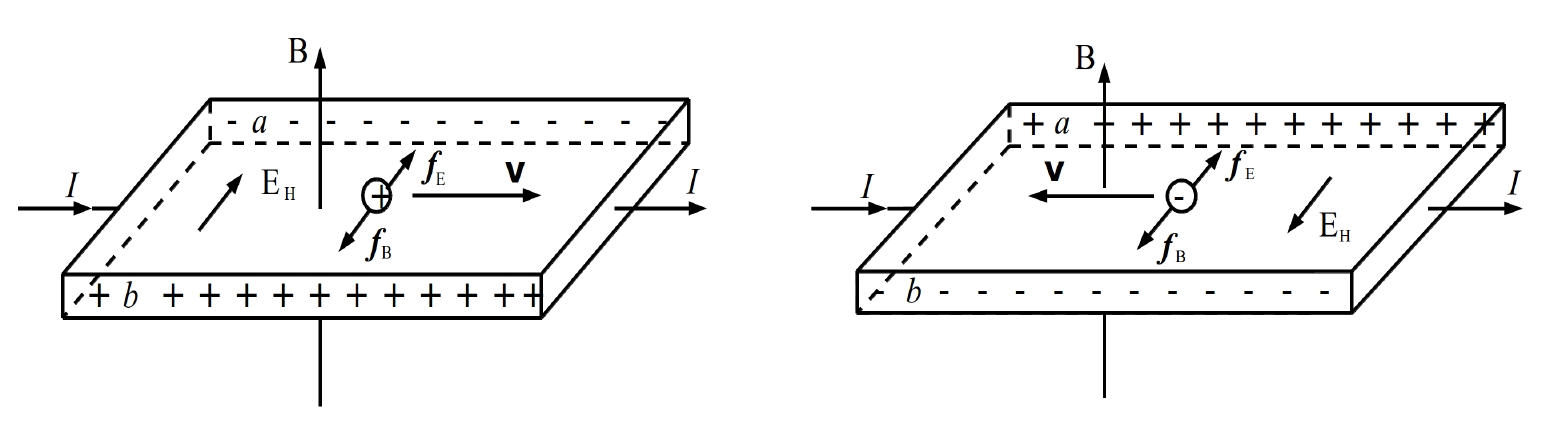
\includegraphics[scale=0.8]{principle.png}
\caption{The principle of the Hall effect.}\label{FigPrinciple}
\end{figure}


	\subsection{Integrated Hall Probe}

Usually, the Hall voltage is very small, therefore it need to be amplified before  measurements. An integrated Hall probe, consisting of a Hall sensor, an amplifier, and a voltage compensator (Figure \ref{FigCircuit}), can be used to amplify the voltage appropriately. 

\begin{figure}[H]
\centering
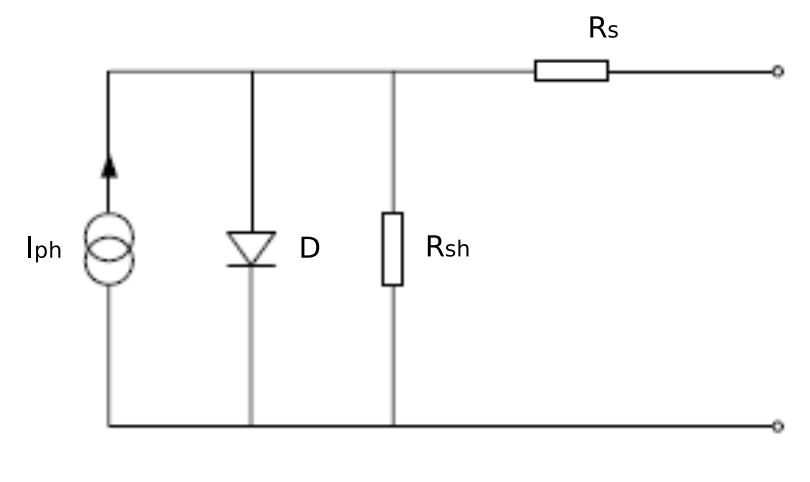
\includegraphics[scale=1.2]{circuit.png}
\caption{The integrated Hall probe SS495A (left). The relation between the output voltage $U$ and the magnitude of the magnetic field $B$ (right).}\label{FigCircuit}
\end{figure}

Hall probe satisfies the following equation:
\begin{equation}\label{eqB}
B = \frac{U-U_0}{K_\text{H}}
\end{equation}
where $U_0$ is the output voltage when the magnetic field is zero.


	\subsection{Magnetic Field Distribution Inside a Solenoid}
The theoretical value of magnetic field distribution on the axis of a single layer solenoid can be calculated using the following formula:

According to the following formula,

\begin{equation}\label{eqBx}
B(x) = \mu_0\frac{N}{L}I_\text{M}\{\frac{L+2x}{2[D^2+(L+2x)^2]^{\frac{1}{2}}}+\frac{L-2x}{2[D^2+(L-2x)^2]^{\frac{1}{2}}}\} = C(x)I_\text{M},
\end{equation}
where $N$ is the number of turns of the solenoid, $L$ is its length, $I_\text{M}$ is the current through the solenoid wire, and D is the solenoid's diameter, $\mu_0 = 4\pi \times 10^{-7} \text{H}/\text{m}.$ is the magnetic permeability of vacuum, the theoretical value of magnetic field distribution on the axis of a single layer solenoid can be calculated. 

The solenoid used in this lab is of 10 layers. Then the net magnetic on the axis of the solenoid can be found by superposition method. The theoretical value of the magnetic field inside the solenoid with $I_\text{M}$ = 0.1 A is given in Table \ref{TableTheoB}.

\begin{table}[H]
\centering
\begin{tabular}{cc||cc}
\toprule
$x$ [cm] & $B$ [mT] & $x$ [cm] & $B$ [mT]\\
\hline
$\pm$ 0.0 & 1.4366 & $\pm$ 8.0 & 1.4057\\
$\pm$ 1.0 & 1.4363 & $\pm$ 9.0 & 1.3856\\
$\pm$ 2.0 & 1.4356 & $\pm$ 10.0 & 1.3478\\
$\pm$ 3.0 & 1.4343 & $\pm$ 11.0 & 1.2685\\
$\pm$ 4.0 & 1.4323 & $\pm$ 11.5 & 1.1963\\
$\pm$ 5.0 & 1.4292 & $\pm$ 12.0 & 1.0863\\
$\pm$ 6.0 & 1.4245 & $\pm$ 12.5 & 0.9261\\
$\pm$ 7.0 & 1.4173 & $\pm$ 13.0 & 0.7233\\
\bottomrule
\end{tabular}
 \caption{Theoretical value of the magnetic field inside the solenoid.}\label{TableTheoB}
\end{table}


		\section{Experimental Setup}

The experimental setup (Figure \ref{FigSetup}) consists of an integrated Hall probe SS495A (b) with $K_\text{H}$ = 31.25 $\pm$ 1.25 V/T (at the working voltage 5$\,$V) or $K_\text{H} = 3.125\pm0.125$ mV/G, a solenoid, a power supply, a voltmeter, a DC voltage divider, and a set of connecting wires. The precisions of the devices are shown in Table \ref{tablePrecision}.

\begin{figure}[H]
    \centering
        \subfigure[Measurement setup]
        {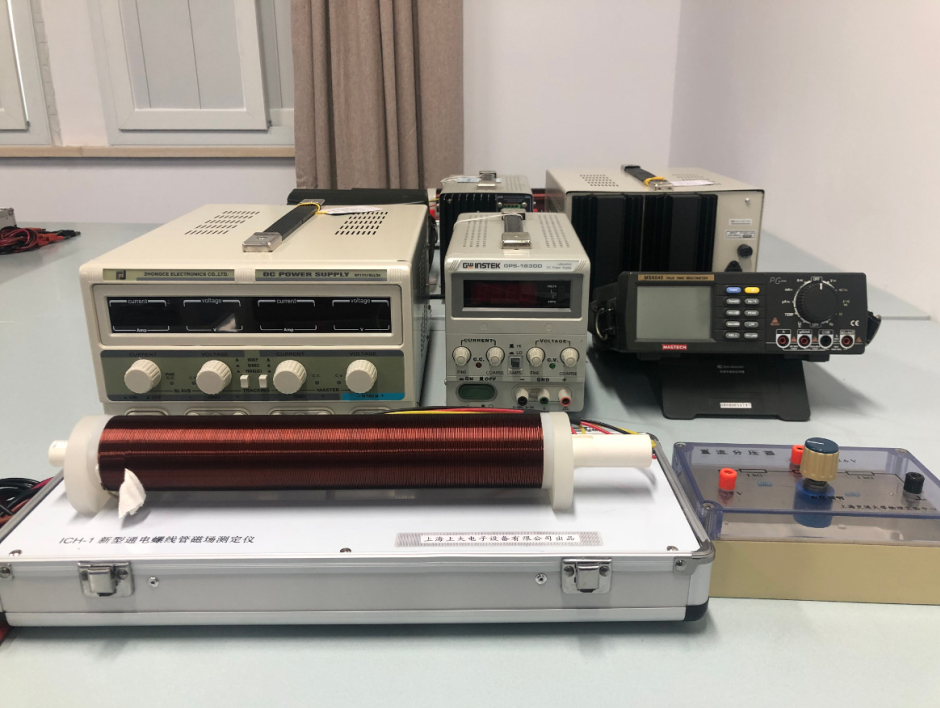
\includegraphics[width=0.45\hsize]{setup.png}}  
        \subfigure[Integrated Hall probe SS495A]
        {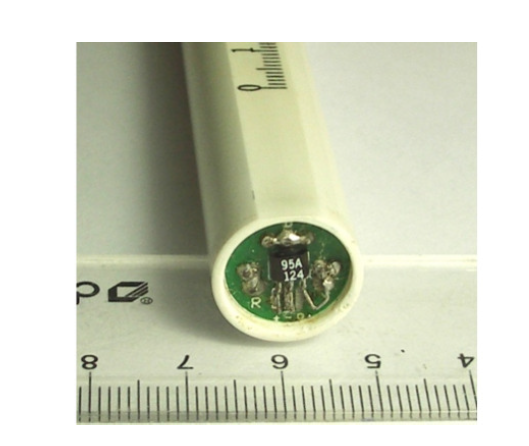
\includegraphics[width=0.45\hsize]{probe.png}} 
         \caption{Experimental setup}
          \label{FigSetup}
\end{figure}

\begin{table}[htbp]
\centering
\begin{tabular}{ccc}
\toprule
Instrument & Measured quantities & Uncertainties \\ 
\hline
Voltage source & Working voltage $U_{s}$ & $0.5\%\,$V \\ 
Multimeter & Output voltage $U_{0}, U$ & $0.05\% + 6\times 10^{-3} or 10^{-4}\,$V \\ 
Current source & Current $I_{0}, I_{M}$ & $2\%\,$mA \\ 
Graduated ruler & Distance & $0.05\,$cm \\
\bottomrule
\end{tabular}
\caption{Information of measurement instruments.}\label{tablePrecision}
\end{table}



		\section{Measurement Procedure}
		
	\subsection{Relation Between Sensitivity $K_\text{H}$ and Working Voltage $U_\text{S}$\label{proc}}
	
In this part, the relation between sensitivity $K_{H}$ and working voltage $U_{S}$ is studied.

First, the integrated Hall probe is placed at the center of the solenoid. Then the working voltage is set at 5V and the output voltage $U_0$ ($I_\text{M}$ = 0) and $U$ ($I_\text{M}$ = 250 mA) are measured through voltage meter.  The sensitivity of the probe $K_\text{H}$ is calculated using Eq. (\ref{eqB}) with theoretical value of $B(x = 0)$ from Table \ref{TableTheoB}.

Then for different values of $U_\text{S}$ (from 2.5 V to 10 V), corresponding $K_\text{H}$ is measured. Then $K_\text{H}/U_\text{S}$ can be obtained and plotted as the curve $K_\text{H}/U_\text{S}$ vs. $U_\text{S}$.


	\subsection{Relation Between Output Voltage $U$ and Magnetic Field $B$}

In this part, the relation between the output voltage of the Hall probe and the magnetic field is verified. 

First, with $B=0$, $U_\text{S}$ = 5V, the 2.4 $\sim$ 2.6 V output terminal of the DC voltage divider is connected to the negative port of the voltmeter, and the voltage is adjusted by spinning the node on the divider until $U_0$ = 0.

Next, the integrated Hall probe is placed at the center of the solenoid.  Then the output voltage $U$ for different values of $I_\text{M}$ ranging from 0 to 500 mA with intervals of 50 mA is measured.

Note that the output voltage $U$ is the amplified signal from $U_\text{H}$.

Then the curve $U$ vs. $B$ is plotted and the sensitivity $K_\text{H}$ can be found out.The value is compared with the theoretical value given in the Apparatus section.

	\subsection{Magnetic Field Distribution Inside the Solenoid}

In this part, the magnetic field distribution inside the solenoid is studied.

With the circuit unchanged and current set to be 250 mA, the position of the Hall probe inside the solenoid is changed in the range of $0\sim30$ cm. The distance of the Hall probe $x$ and corresponding output voltage $U$ are recorded. With $K_H$ found by previous experiment, a curve of $B = B(x)$ can be plotted with the aid of computer.

\newpage

		\section{Results}
		
	\subsection{Relation Between Sensitivity $K_\text{H}$ and Working Voltage $U_\text{S}$}
	
	The measurement results of $U_0$ and $U$ when $U_\text{S}$ = 4.99 V are shown in Table \ref{TableU5}.

\begin{table}[H]
\centering
\begin{tabular}{c|c|c}
\toprule
$U_\text{S} \,\,[\text{V}] \pm 0.5\%\,\,[\text{V}]$ & $U_0 (I_\text{M} = 0) \,\,[\text{V}] \pm (0.05\% + 6\times10^{-3} )\,\,[\text{V}]$ & $U (I_\text{M} = 250\,\text{mA}) \,\,[\text{V}] \pm (0.05\% + 6\times10^{-3}) \,\,[\text{V}]$\\
\midrule
4.99  & 2.477  & 2.597 \\
\bottomrule
\end{tabular}
\caption{Data for $U_0$ and $U$ with $U_\text{S}$ = 5 V.}\label{TableU5}
\end{table}

According to the data in Table \ref{TableTheoB}, when $I_\text{M} = 100 \,\,\text{mA},$ $B(x=0,I_\text{M}=100\,\text{mA})=1.4366\times10^{-3}\,\,\text{T}.$
From Eq. (\ref{eqBx}), $B$ is proportional to current $I_\text{M}$, which yields 
$$B(x=0,I_\text{M}=250\,\text{mA}) = \frac{250}{100} \times 1.4366\times10^{-3} = 3.5915\times 10^{-3}\,\,\text{T}.$$

According to Eq. (\ref{eqB}), the sensitivity of the probe $K_\text{H}$ when $U_\text{S}$ = 4.99 V is:
$$K_\text{H} = \frac{U-U_0}{B(x=0,I_\text{M}=250\,[\text{mA}])} = \frac{2.597-2.477}{3.5915\times 10^{-3}} = 33 \pm 3 \,[\text{V}/\text{T}]~~~~u_{r,K_H} = 9\%
$$

\begin{table}[!ht]
    \centering
    \begin{tabular}{ccccc}
    \toprule
        ~ & $U_S [V] \pm 0.5\% [V]$ & $U_0 \pm 0.05\% + 6\times 10^{-3/-4} [V] $ & $U_0 \pm 0.05\% + 6\times 10^{-3/-4} [V] $ & $K_H/U_S [T^{-1}]$  \\ \midrule
        1  & 2.80 & 1.3882 & 1.4575 & 6.9 \\
2  & 3.20 & 1.5883 & 1.6667 & 6.8 \\
3  & 3.60 & 1.7856 & 1.8735 & 6.8 \\
4  & 4.00 & 1.9835 & 2.0826 & 6.9 \\
5  & 4.40 & 2.183  & 2.289  & 6.7 \\
6  & 4.80 & 2.381  & 2.495  & 6.6 \\
7  & 5.20 & 2.578  & 2.700  & 6.5 \\
8  & 5.60 & 2.774  & 2.902  & 6.4 \\
9  & 6.00 & 2.971  & 3.106  & 6.3 \\
10 & 6.40 & 3.174  & 3.314  & 6.1 \\
11 & 6.80 & 3.366  & 3.509  & 5.9 \\
12 & 7.20 & 3.560  & 3.705  & 5.6 \\
13 & 7.60 & 3.753  & 3.902  & 5.5 \\
14 & 8.00 & 3.953  & 4.104  & 5.3 \\
15 & 8.40 & 4.144  & 4.300  & 5.2 \\
16 & 8.80 & 4.339  & 4.496  & 5.0 \\
17 & 9.20 & 4.532  & 4.687  & 4.7 \\
18 & 9.60 & 4.726  & 4.882  & 4.5 \\ \bottomrule
    \end{tabular}
    \caption{Table for $U_0$ and $U$ with different $U_S$} \label{Tab2}
\end{table}

The measurement results of $U_0$ and $U$ for different $U_\text{S}$ as well as their corresponding ratio are shown in Table \ref{Tab2}.  For each set of data, the ratio of $K_H$ and $U_S$ is calculated as
$$\displaystyle \frac{K_\text{H}}{U_\text{S}} = \frac{U-U_0}{BU_\text{S}}.$$
Take the first set of data as an example,
$$\frac{K_\text{H}}{U_\text{S}} = \frac{U-U_0}{BU_\text{S}} = \frac{1.4575-1.3882}{3.5915\times 10^{-3}\times2.80} =  6.9 \pm 0.2 \,[\text{T}^{-1}]~~~~u_{r,K_H/U_S} = 3\%$$
A plot of the results $K_\text{H}/U_\text{S}$ vs. $U_\text{S}$ using \textit{\textbf{Origin}} is shown in Figure \ref{FigKU}.

\begin{figure}[H]
\centering
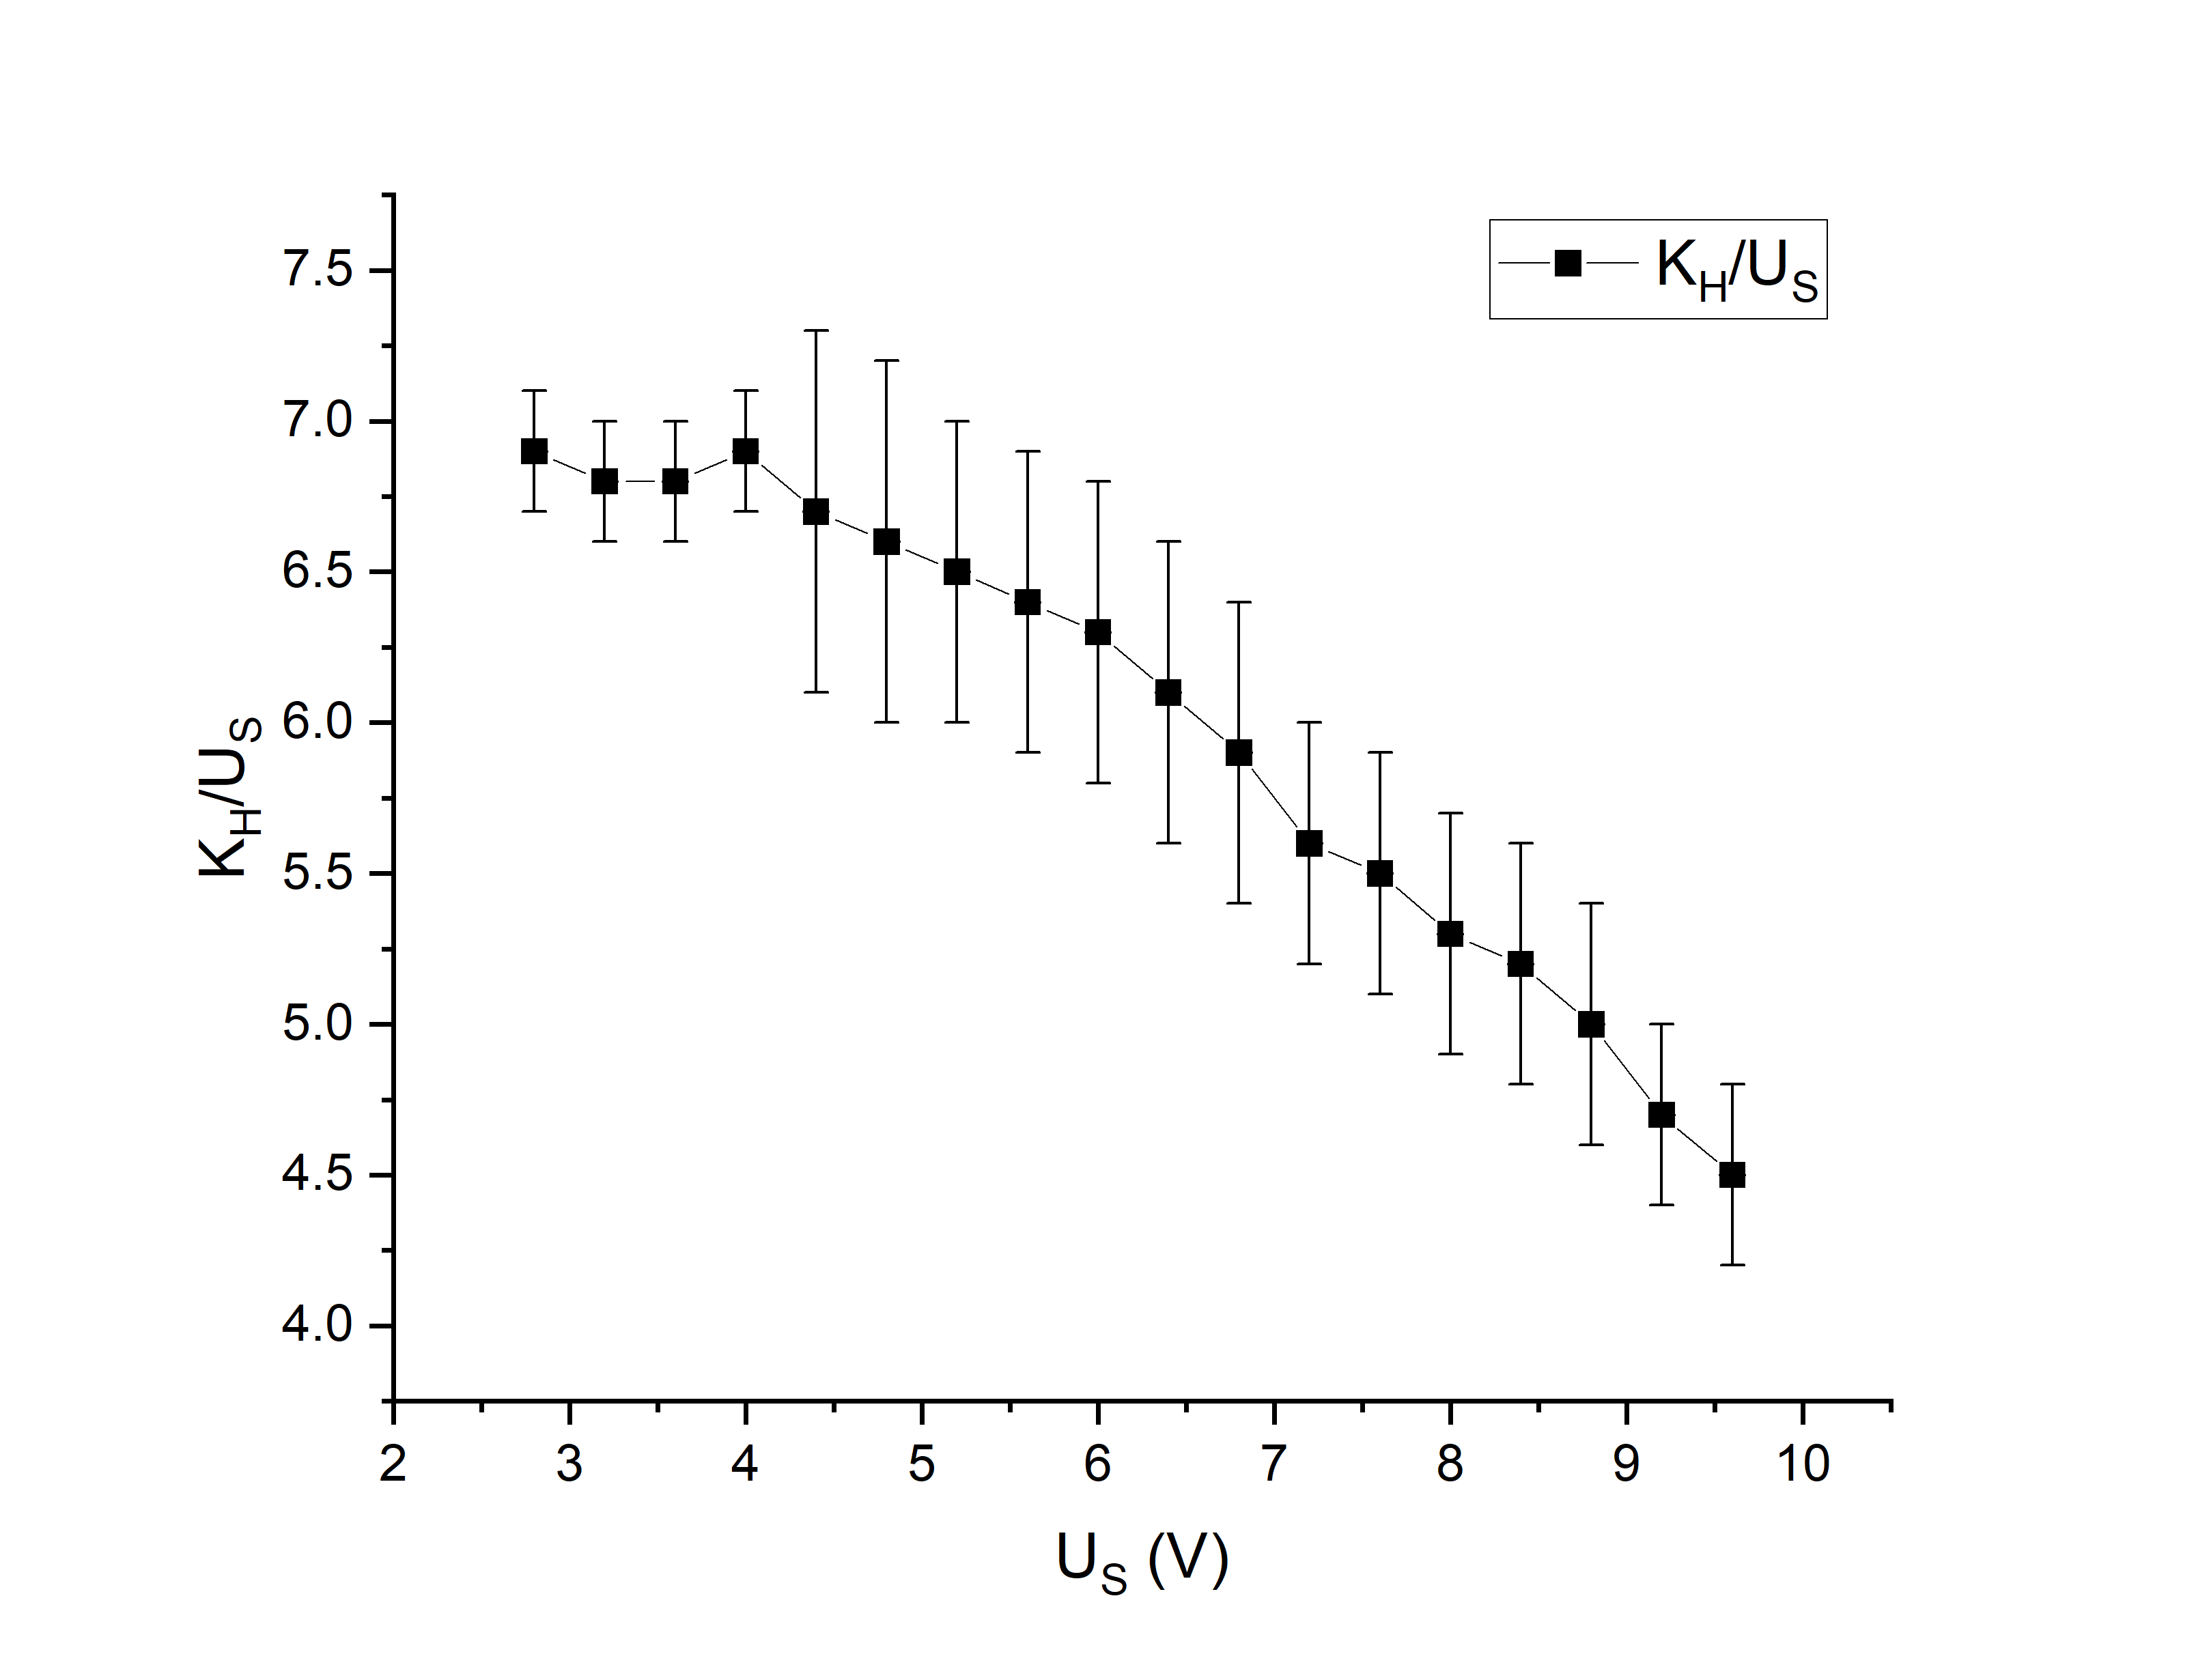
\includegraphics[scale=0.5]{K-U.png}
\caption{The $K_\text{H}/U_\text{S}$ vs. $U_\text{S}$ relation.}\label{FigKU}
\end{figure}

\textbf{The points in the plot indicates that, generally,  the ratio of $K_{H}$ to $U_{s}$ decreases as $U_{s}$ increases.}

	\subsection{Relation Between Output Voltage $U$ and Magnetic Field $B$}\label{SecUB}
	
According to Eq. (\ref{eqBx}), $B$ is proportional to the current $I_\text{M}$. Therefore, the theoretical value of the magnetic field is $$B(x=0) = \frac{I_\text{M}}{100}\times 1.4366\times10^{-3}.$$
Take the second set of data as an example, 
$$B(x=0,I_\text{M}=50\,[\text{mA}]) = \frac{1.4366\times10^{-3}}{100}\times I_\text{M} = 0.718\times 10^{-3}\,[\text{T}].$$
However, the value of $U$ is the amplified signal from output $U_H$. therefore, 
$$B(x=0) = \frac{U-U_0}{K_\text{H}} = \frac{U}{K_\text{H}} = k\cdot\frac{U_\text{H}}{K_\text{H}},$$
where $k$ is a constant that will not affect the results.

The experimental results and corresponding magnetic field $B$ are shown in Table \ref{TableI}. Using linear fit to obtain the $I_\text{M}$ vs. $U$ curve (Figure \ref{FigUB}), sensitivity can be expressed by the slope of the curve $K_{H}= 31.9\, \pm 0.3\,$V/T.

\begin{table}[H]
\centering
\begin{tabular}{cccc}
\toprule
& $I_\text{M}\,\,[\text{mA}] \pm 2\%\,\,[\text{mA}]$ & $B(x=0)\,\,\,\text{mT}]$ & $U\,\,[\text{mV}]\pm (0.05\%+0.6/0.06))\,\,[\text{mV}]$\\
\midrule
1 & 0  & 0 & 0.00  \\
2 & 50  & 0.718  & 30.00  \\
3 & 100  & 1.44 & 51.00  \\
4 & 150  & 2.16  & 74.50  \\
5 & 200  & 2.87 & 95.00  \\
6 & 250  & 3.59  & 120.00  \\
7 & 300 & 4.31  & 142.60  \\
8 & 350  & 5.03  & 166.00  \\
9 & 400  & 5.75  & 187.00  \\
10 & 450 & 6.47  & 209.60  \\
11 & 500 & 7.18 & 233.3  \\
\bottomrule
\end{tabular}
\caption{Measurement data for the $I_\text{M}$ vs. $U$ relation and the calculated data for $B(x=0)$.}\label{TableI}
\end{table}

\begin{figure}[H]
\centering
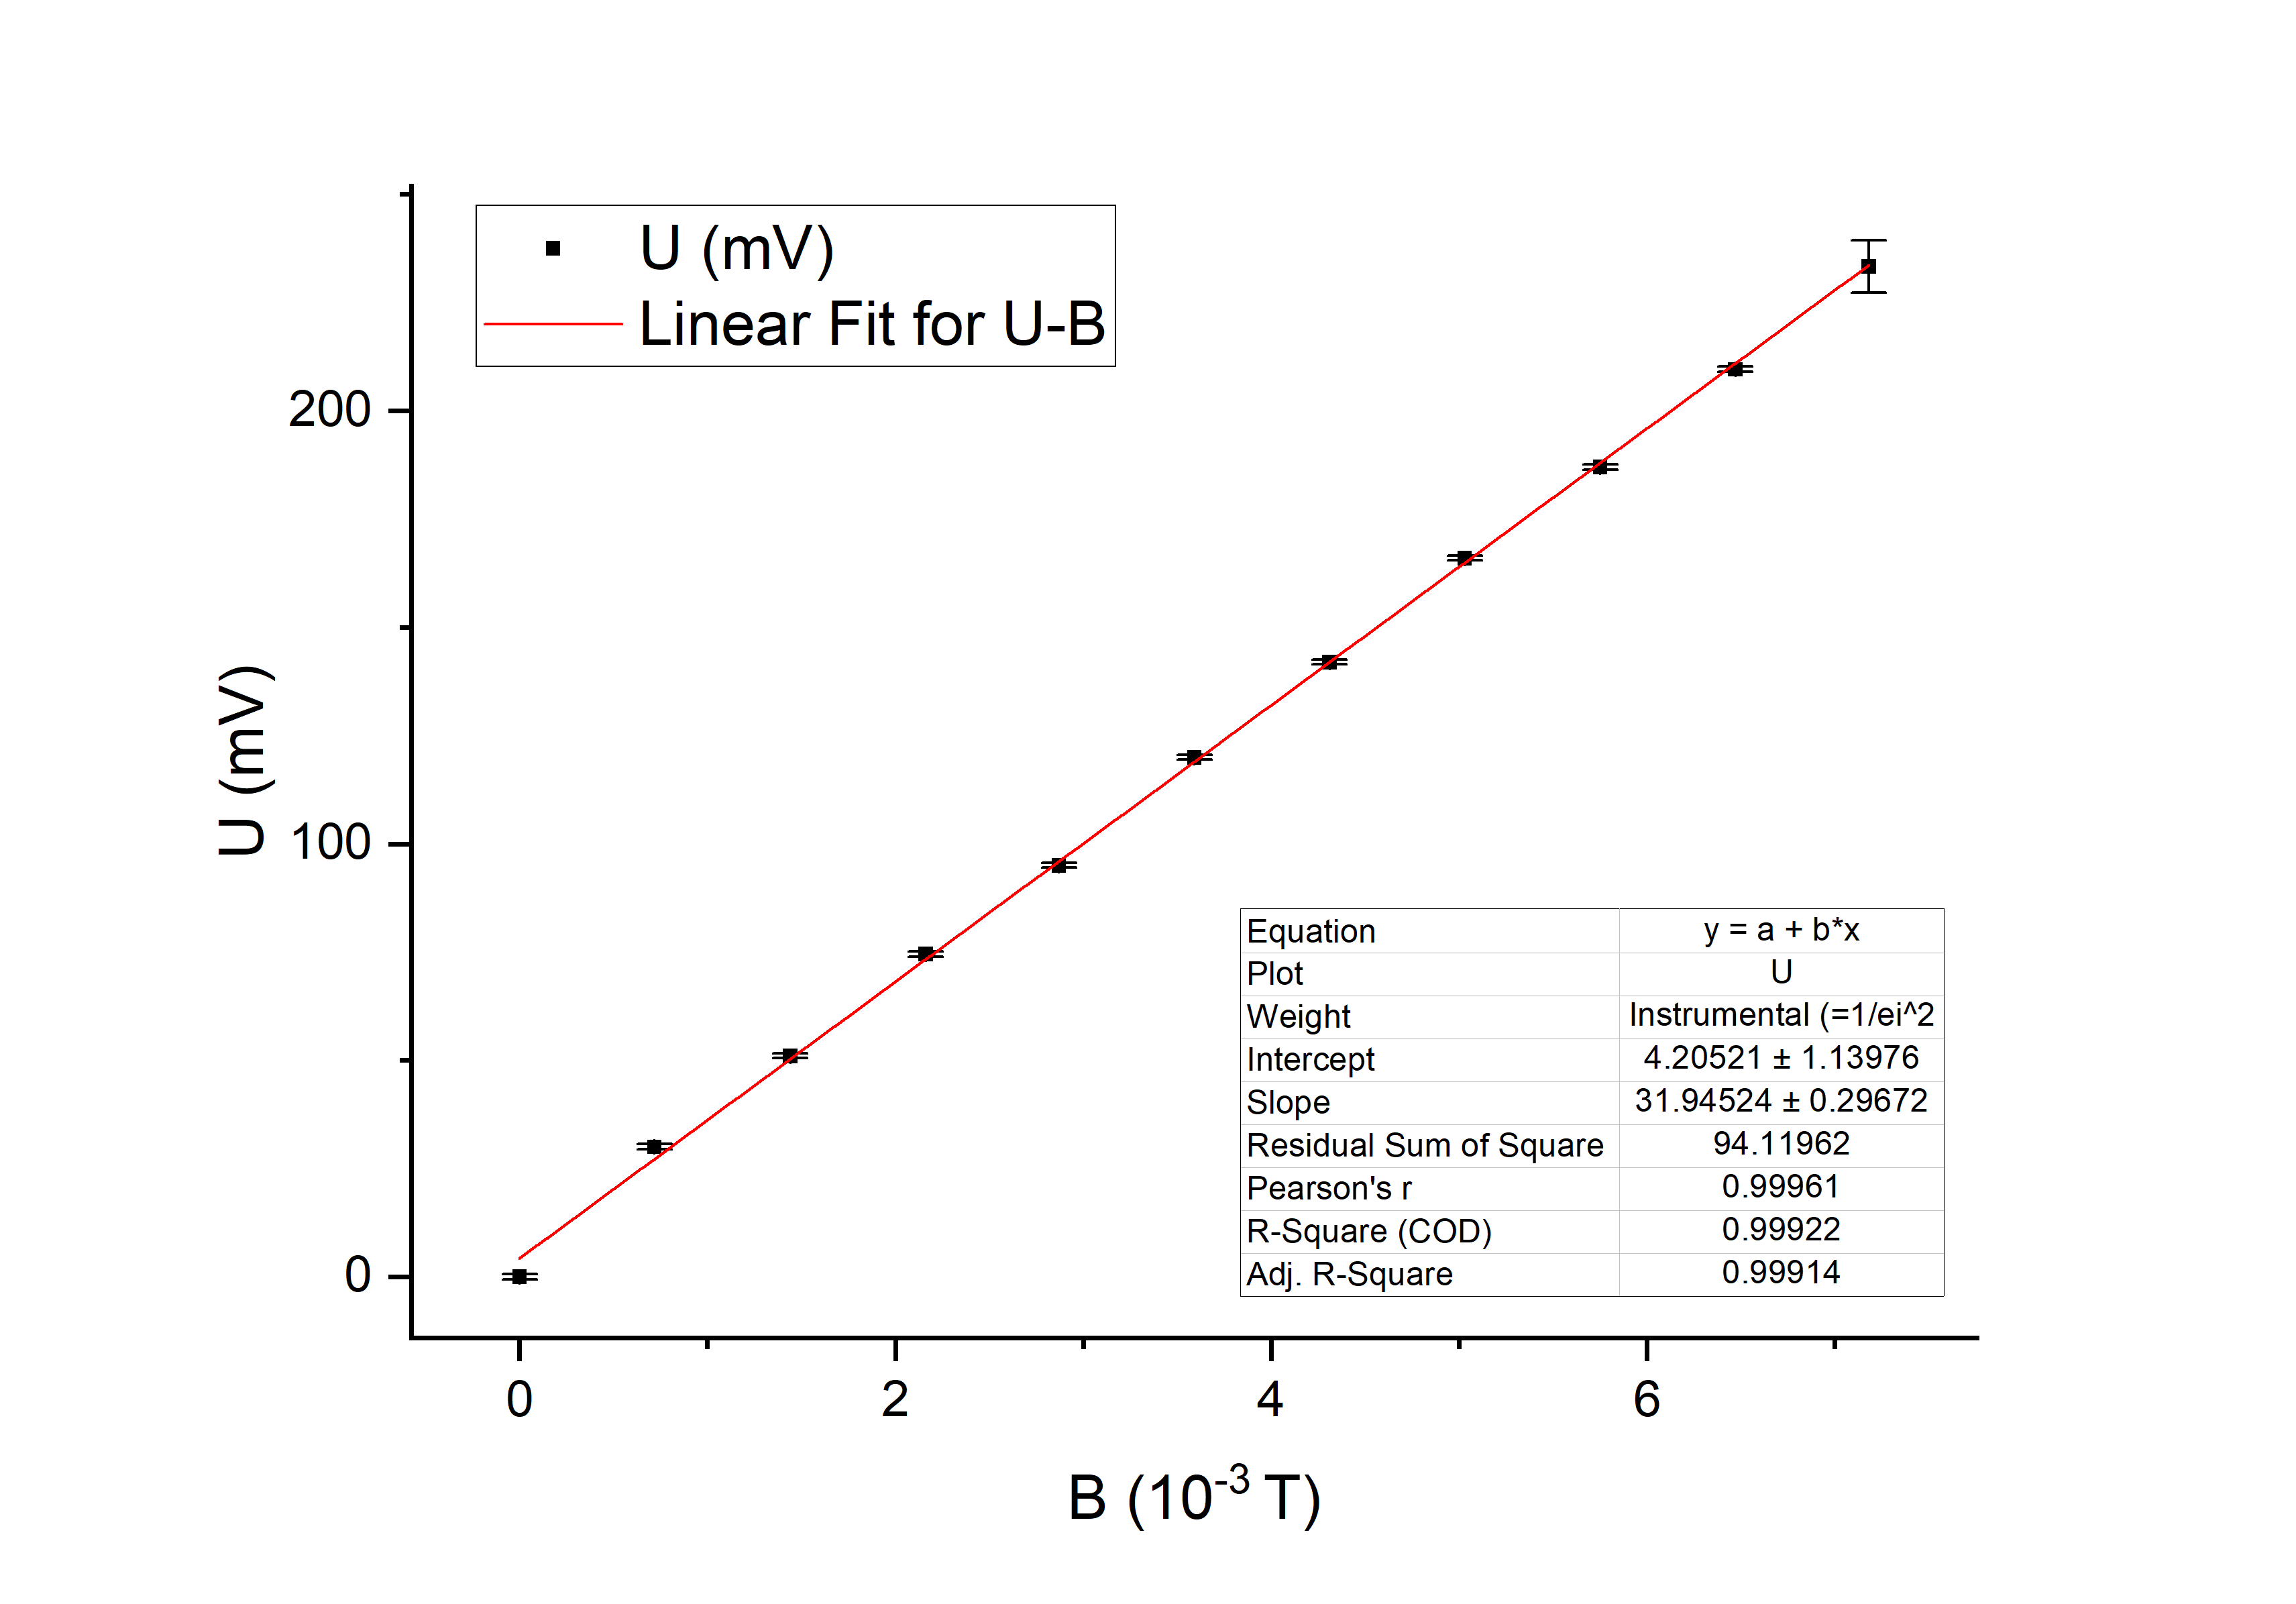
\includegraphics[scale=0.5]{U-B.png}
\caption{The linear fit of $U$ vs. $B$ relation.}\label{FigUB}
\end{figure}

	\subsection{Magnetic Field Distribution Inside the Solenoid}

According to Eq.\eqref{eqB} and the experimental result of $K_{H}$ from section \ref{SecUB}, $B(x)$ can be calculated by 
$$\displaystyle B(x) = \frac{U}{K_\text{H}} = \frac{U}{31.9} .$$ 
The measurement result of output voltage $U$ and the corresponding position $x$ are shown in Table \ref{Tab.xUB}. 
Take the first set of data as an example, $$B(x) = \frac{U}{31.9} = \frac{10.40}{31.9} = (0.33 \pm 0.02) \,[\text{mT}]~~~~u_{r,B(x)} = 6\%$$ 
Other values are shown in Table \ref{Tab.xUB}.

\begin{table}[H]
\centering
\begin{tabular}{cccc||cccc}
\toprule
   & x[cm]   & U[mV]    & $B(x)$    &    & x[cm]   & U[mV]  & $B(x)$   \\
   & $\pm$ 0.05[cm]    & $\pm \, (0.05\%+0.06)$[mV]      & [mT]    &    & $\pm$ 0.05[cm]    & $\pm \, (0.05\%+0.06)$[mV]       & [mT]   \\ \midrule
1  & 0.00  & 10.40  & 0.33 & 27 & 15.60 & 118.68 & 3.72 \\
2  & 0.60  & 14.11  & 0.44 & 28 & 16.20 & 118.80 & 3.72 \\
3  & 1.20  & 20.60  & 0.65 & 29 & 16.80 & 118.83 & 3.73 \\
4  & 1.80  & 30.75  & 0.96 & 30 & 17.40 & 118.90 & 3.73 \\
5  & 2.40  & 47.60  & 1.49 & 31 & 18.00 & 118.88 & 3.73 \\
6  & 3.00  & 68.50  & 2.15 & 32 & 18.60 & 118.92 & 3.73 \\
7  & 3.60  & 86.24  & 2.70 & 33 & 19.20 & 119.75 & 3.75 \\
8  & 4.20  & 98.20  & 3.08 & 34 & 19.80 & 118.60 & 3.72 \\
9  & 4.80  & 105.50 & 3.31 & 35 & 20.40 & 118.50 & 3.71 \\
10 & 5.40  & 110.00 & 3.45 & 36 & 21.00 & 118.40 & 3.71 \\
11 & 6.00  & 112.60 & 3.53 & 37 & 21.60 & 118.00 & 3.70 \\
12 & 6.60  & 114.55 & 3.59 & 38 & 22.20 & 117.71 & 3.69 \\
13 & 7.20  & 115.60 & 3.62 & 39 & 22.80 & 117.32 & 3.68 \\
14 & 7.80  & 116.60 & 3.66 & 40 & 23.40 & 116.83 & 3.66 \\
15 & 8.40  & 117.10 & 3.67 & 41 & 24.00 & 111.70 & 3.50 \\
16 & 9.00  & 117.70 & 3.69 & 42 & 24.60 & 115.13 & 3.61 \\
17 & 9.60  & 118.00 & 3.70 & 43 & 25.20 & 113.83 & 3.57 \\
18 & 10.20 & 118.30 & 3.71 & 44 & 25.80 & 111.70 & 3.50 \\
19 & 10.80 & 118.50 & 3.71 & 45 & 26.40 & 108.33 & 3.40 \\
20 & 11.40 & 118.55 & 3.72 & 46 & 27.00 & 102.43 & 3.21 \\
21 & 12.00 & 118.70 & 3.72 & 47 & 27.60 & 93.55  & 2.93 \\
22 & 12.60 & 118.80 & 3.72 & 48 & 28.20 & 78.60  & 2.46 \\
23 & 13.20 & 118.80 & 3.72 & 49 & 28.80 & 59.65  & 1.87 \\
24 & 13.80 & 118.79 & 3.72 & 50 & 29.40 & 39.76  & 1.25 \\
25 & 14.40 & 118.65 & 3.72 & 51 & 30.00 & 25.73  & 0.81 \\
26 & 15.00 & 118.70 & 3.72 &    &       &        &         \\  \bottomrule
\end{tabular}
\caption{Table of $x$, $U$ and $B(x)$}\label{Tab.xUB}
\end{table}


The theoretical curve of the magnetic field distribution inside the solenoid can be plotted using data in Table \ref{TableTheoB}. According to $B(x) = C(x)I_M$, magnetic filed should be proportional to the current.Therefore, the values in Table \ref{TableTheoB} need to be multiplied by $\frac{250}{100}$, because in this sub-experiment, the current is 250 mA instead of 100 mA. 

Next, using \textbf{\textit{Origin}}, the curves of experimental and theoretical distribution of magnetic field in a solenoid is plotted together, as is shown in Figure \ref{FigB}.

\begin{figure}[H]\centering
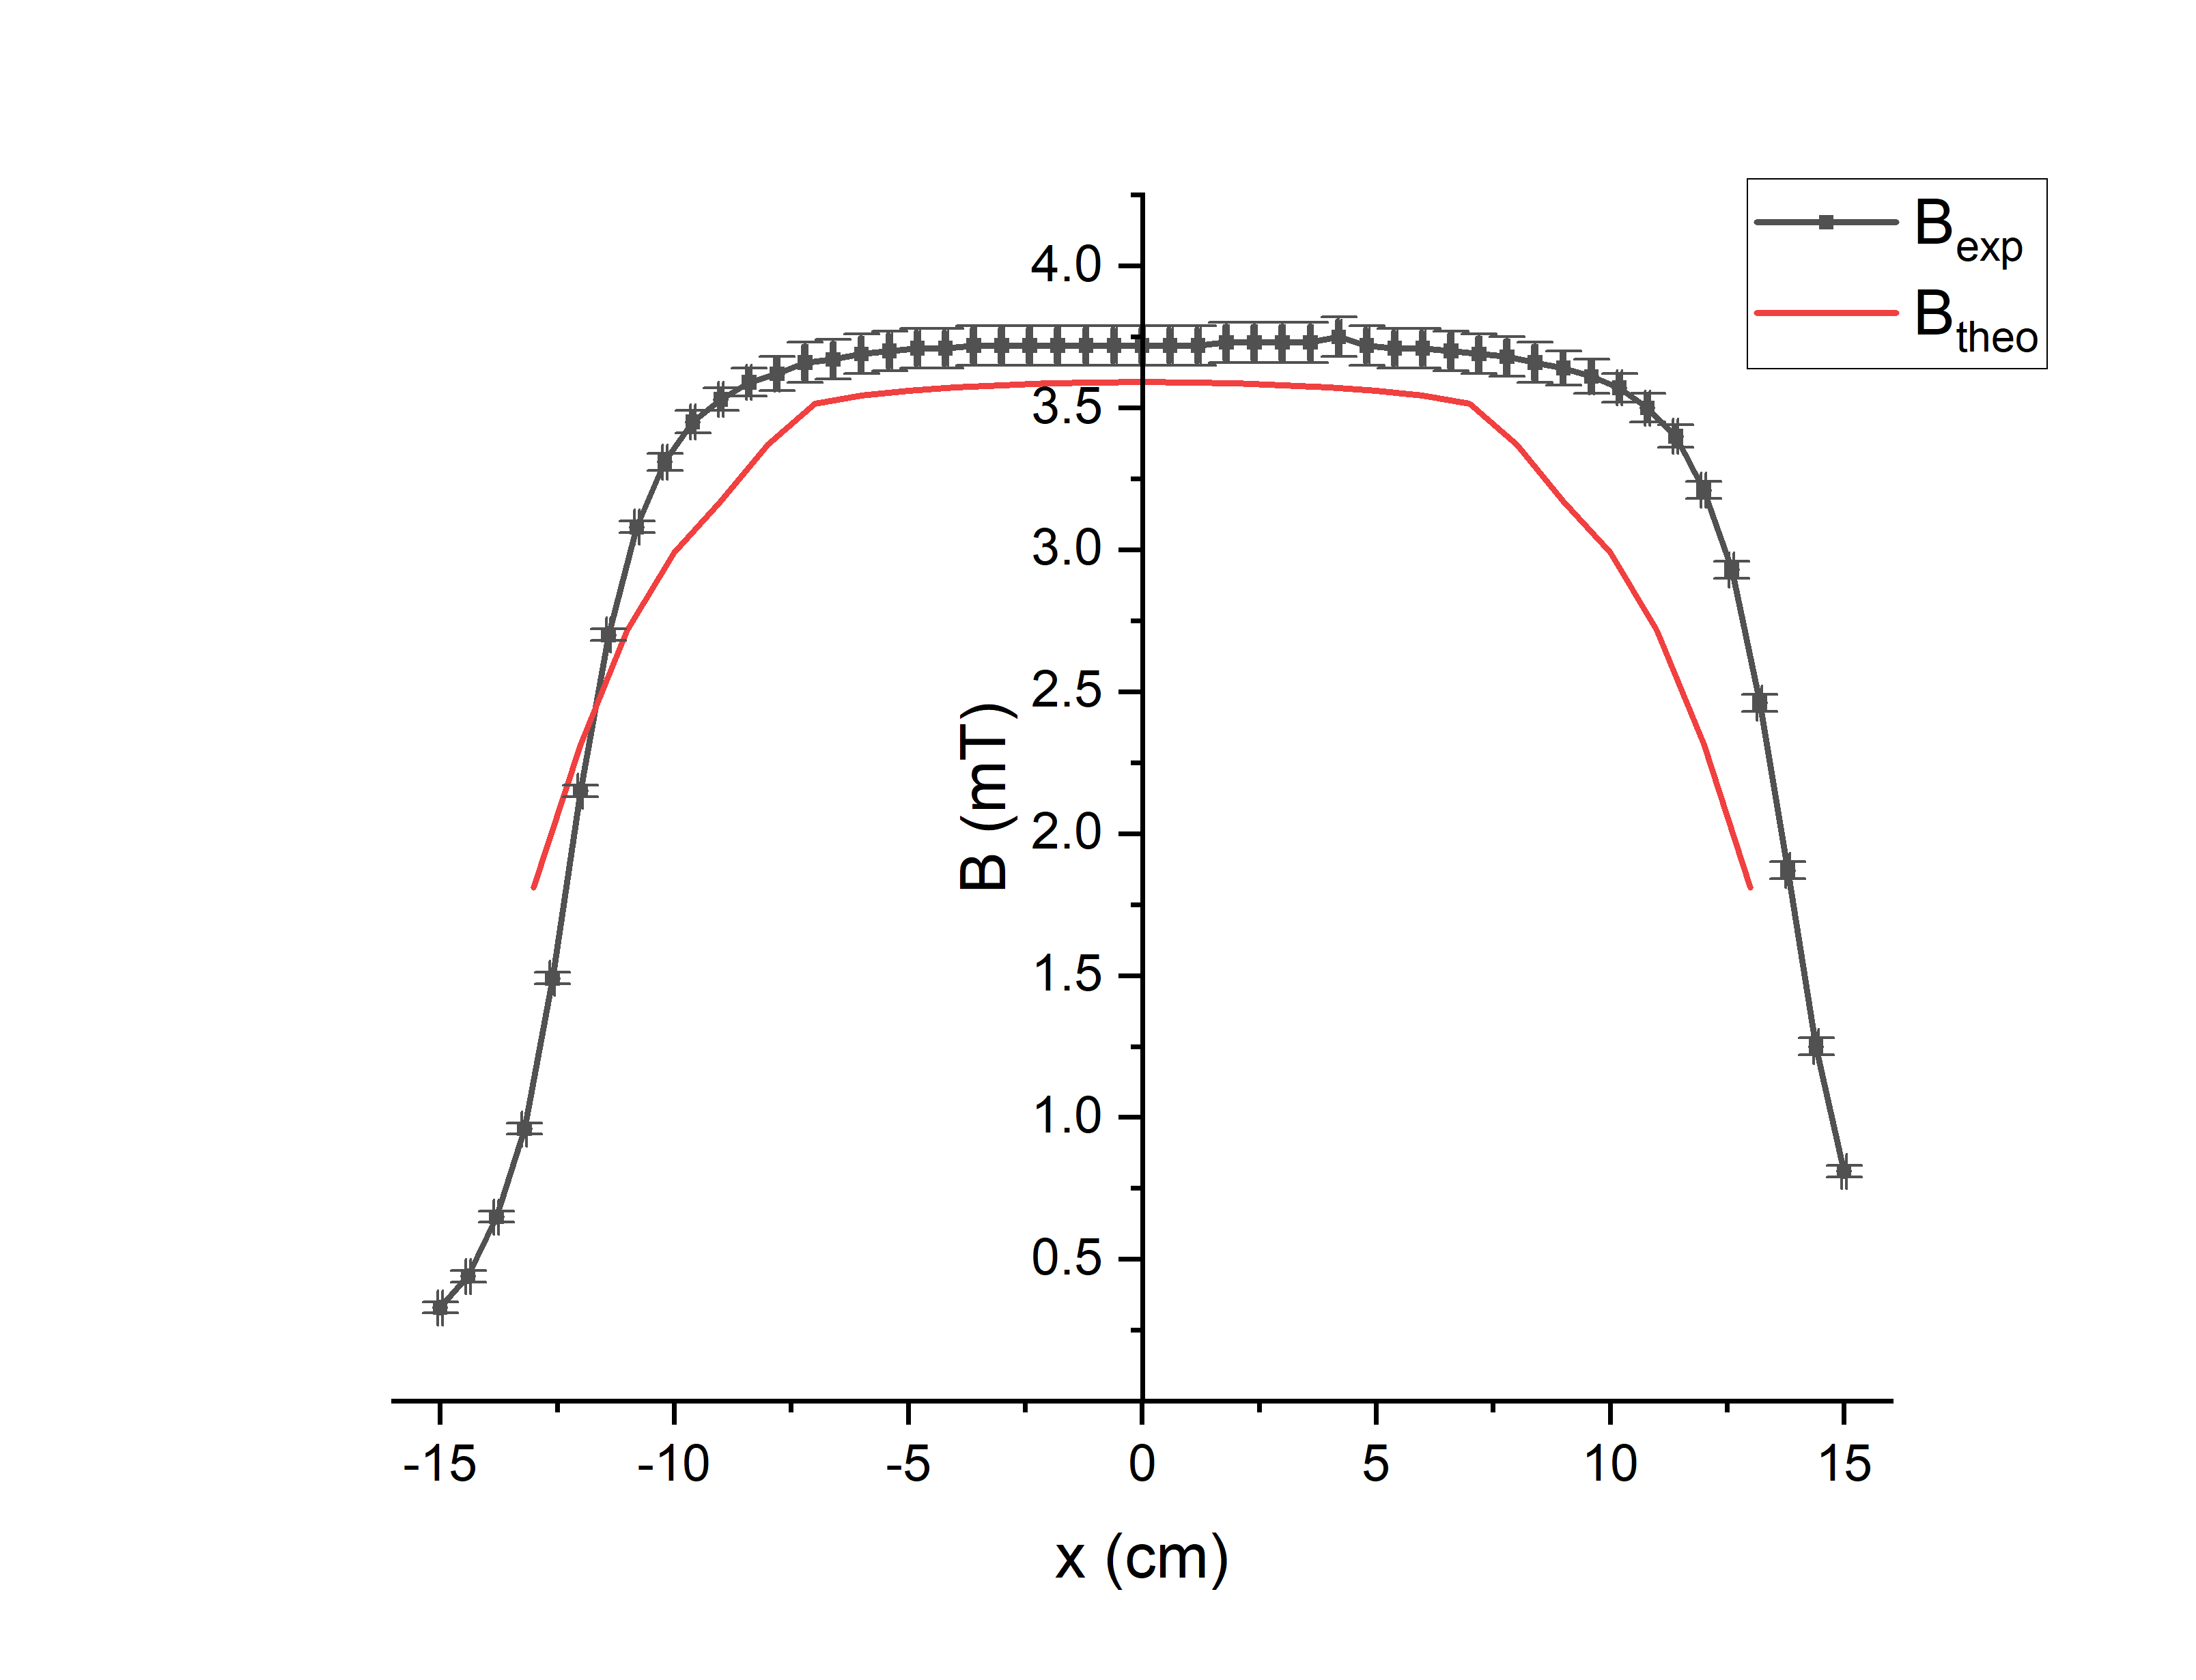
\includegraphics[scale=0.5]{B-comp.png}
\caption{Measured and theoretical magnetic field distribution inside the solenoid.}\label{FigB}
\end{figure}

		\section{Conclusions and Discussion}
		
	\subsection{Relation Between Sensitivity $K_\text{H}$ and Working Voltage $U_\text{S}$}

In this part, the relation between sensitivity $K_\text{H}$ and working voltage $U_\text{S}$ is studied. From Figure \ref{FigKU}, the curve shows a trend that the ratio of sensitivity $K_H$ to working voltage $U_S$ and working voltage $U_\text{S}$ has a negative correlation in general. In other words, the ratio decreases as working voltage increases.

The theoretical value of $K_H$ is 31.25 V/T according to [1]. Therefore the deviation between theoretical value and experimental value is 5\%, which is relatively small.

Moreover, the plot shows that the ratio decreases almost uniformly when $U_S$ becomes greater than 5, indicating that $K_H$ remains nearly constant as $U_S$ increases. As for the points whose $U_S$ are less than 5, they behave irregularly. This behaviour verifies the working voltage of the Hall probe to be 5 V, exceeding which can the Hall probe work properly. Therefore, this experiment is considered to be successful, as the experimental critical  working voltage match with the theoretical one.
	
	\subsection{Relation Between Output Voltage $U$ and Magnetic Field $B$}
	
In this part, the relation between output voltage and magnetic field is studied. According to the linear fit curve and corresponding Pearson's r (0.99961), it implies that these two parameters are likely to be linear dependent. Notice that the intercept of the curve is 4.21, which is relatively small compared to the voltage $U$, therefore it can be further deduced that the output voltage is proportional to the magnetic field. This conclusion also fits with the conclusion from section 1 that  $K_H$ remains nearly constant as $U_S$ increases.

The slope of the linear fit indicates that the sensitivity $K_H$ is  31.9 V/T. Compared with the theoretical value $K_{theo}=31.25$ V/T, the experimental result has relative error
$$
U_{r,K_\text{H}} = \frac{31.9-31.25}{31.25}\times 100\% = 2.3\,\%
$$ 
which is of high accuracy.

According to lab manual [1], it is stated that "When the external magnetic field is not too strong, the Hall voltage is proportional to both the current and the magnitude of the magnetic field......". In this lab, given that the current varied from 0-500 mA, some of which might be "too strong" for the Hall element, leading to inaccurate results.
	
	
	
	\subsection{Magnetic Field Distribution Inside the Solenoid}
	
In this part, the distribution of magnetic field inside a solenoid is studied. It can be seen from Figure \ref{FigB} 
that the experimental distribution basically matches with the theoretical distribution, sharing a similar trend. The magnetic field increases rapidly as the distance from the center becomes smaller. After it reaches its maximum, it becomes nearly constant.

However, the two curves still have noticeable deviations all along, and the experimental values are generally bigger than the theoretical values. Possible reason might be:

\begin{enumerate}
\item  The solenoid used in the experiment is denser than expected;
\item The digit displayed on the device is highly unstable, and I tended to read the greater values from it.
\end{enumerate}

		\section{Reference}

\noindent [1] VP241 Exercise 2: The hall probe: characteristics and applications, Shanghai Jiaotong University.

\newpage



\appendix



		\section{Measurement Uncertainty Analysis}

	\subsection{Uncertainty of Sensitivity $K_\text{H}$ and Voltage Measurements}

For Table \ref{TableU5}, the uncertainties can be calculated as
$$u_{U_\text{S}} = 4.99\times 0.5\% \approx 0.03\,\,[\text{V}]~~~~u_{r,U_S} = 0.5\%$$
$$u_{U_0} = 2.477\times0.05\%+6\times10^{-3} \approx 0.007\,\,[\text{V}]~~~~u_{r,U_0} = 0.03\%$$
$$u_U = 2.597\times0.05\%+6\times10^{-3} \approx 0.007\,\,[\text{V}]~~~~u_{r,U} = 0.03\%$$

For $K_\text{H} = \frac{U-U_0}{B}$, its uncertainty is
\begin{align*}
u_{K_\text{H}} &= \sqrt{(\frac{\partial K_\text{H}}{\partial U}u_U)^2+(\frac{\partial K_\text{H}}{\partial U_0}u_{U_0})^2} = \sqrt{(\frac{u_U}{B})^2+(\frac{-u_{U_0}}{B})^2} \\
&=\sqrt{(\frac{0.007}{1.4366\times10^{-3}\times250/100})^2+(\frac{-0.007}{1.4366\times10^{-3}\times250/100})^2} \\&\approx 3\,\,[\text{V}/\text{T}].
\end{align*}


For Table \ref{Tab2}, the uncertainties of data for voltage measurements are calculated as follows. Take the first set of data as an example, 
$$u_{U_\text{S}} = 2.80\times 0.5\% \approx 0.014\,\,[\text{V}]~~~~u_{r,U_S} = 0.5\%$$
$$u_{U_0} = 1.3882\times0.05\%+6\times10^{-4} \approx 0.0013\,\,[\text{V}]~~~~u_{r,U_0} = 0.09\%$$
$$u_U = 1.4575\times0.05\%+6\times10^{-4} \approx 0.0013\,\,[\text{V}]~~~~u_{r,U} = 0.09\%$$

The uncertainty for $ \displaystyle K_\text{H}/U_\text{S} = \frac{U-U_0}{BU_\text{S}}$ is calculated as
\begin{align*}
u_{K_\text{H}/U_\text{S}} &= \sqrt{(\frac{\partial K_\text{H}/U_\text{S}}{\partial U}u_U)^2+(\frac{\partial K_\text{H}/U_\text{S}}{\partial U_0}u_{U_0})^2+(\frac{\partial K_\text{H}/U_\text{S}}{\partial U_\text{S}}u_{U_\text{S}})^2} \\
&= \sqrt{(\frac{u_U}{BU_\text{S}})^2+(\frac{-u_{U_0}}{BU_\text{S}})^2+(-\frac{U-U_0}{BU_\text{S}^2}u_{U_\text{S}})^2} \\
&= \sqrt{(\frac{u_U}{BU_\text{S}})^2+(\frac{-u_{U_0}}{BU_\text{S}})^2+(-\frac{U-U_0}{BU_\text{S}^2}u_{U_\text{S}})^2} \\
&= \sqrt{(\frac{0.0013}{1.4366\times10^{-3}\times250/100\times2.80})^2+(\frac{-0.0013}{1.4366\times10^{-3}\times250/100 \times2.80})^2+(-\frac{1.4575-1.3882}{1.4366\times10^{-3}\times250/100 \times2.80^2}\times0.014)^2} \\
&\approx0.2\,\,[\text{T}^{-1}].
\end{align*}

with relative uncertainty $u_{K_H/U_S} = \frac{0.2}{6.9} \times 100\% = 3\%.$

Other uncertainties are calculated in the same way.

\begin{table}[H]
\centering
\begin{tabular}{crrrc}
\toprule
& $u_{U_\text{S}}\,\,[\text{V}]$ & $u_{U_0}\,\,[\text{V}]$ & $u_U\,\,[\text{V}]$ & $u_{K_\text{H}/U_\text{S}}\,\,[\text{T}^{-1}]$\\
\midrule
  1 & 0.014 & 0.0013 &0.0013 &0.2 \\
  2 & 0.016 & 0.0014 &0.0014 &0.2 \\
  3 & 0.018 & 0.0015 &0.0015 &0.2 \\
  4 & 0.02 & 0.0016 &0.0016 &0.2 \\
  5 & 0.02 & 0.0017& 0.007 & 0.5\\
  6 & 0.02 & 0.007 & 0.007 & 0.6\\
  7 & 0.03 & 0.007 & 0.007 & 0.5\\
  8 & 0.03 & 0.007 & 0.007 & 0.5\\
  9 & 0.03 & 0.007 & 0.008 & 0.5\\
  10 & 0.03 &0.008  &0.008  &0.5 \\
  11 & 0.03 &0.008  &0.008  &0.5 \\
  12 & 0.04 &0.008  &0.008  &0.4 \\
  13 & 0.04 &0.008  &0.008  &0.4 \\
  14 & 0.04 &0.008  &0.008  &0.4 \\
  15 & 0.04 &0.008  &0.008  &0.4 \\
  16 & 0.04 &0.008  &0.008  &0.4 \\
  17 & 0.05 &0.008  &0.008  &0.3 \\
  18 & 0.05 &0.008  &0.008  &0.3 \\
\bottomrule
\end{tabular}
\caption{Uncertainties of data in Table 4.}\label{TableUncK}
\end{table}

	\subsection{Uncertainty of Input Current $I_\text{M}$, Output Voltage $U$ and Magnetic Field $B$}

Take the second set of data in Table \ref{TableI} as an example.\\

The uncertainty for $I_\text{M}$ is
$$u_{I_\text{M}} = 50\times 2\% = 1.0\,\,[\text{mA}]~~~~u_{r,I_M} = 2\%$$

The uncertainty for $U$ is 
$$u_U = 30.00\times 0.05\%+0.6 = 0.6\,\,[\text{mV}]~~~~u_{r,U} = 2\%$$

The uncertainties of all other data are calculated in this way.

\begin{table}[H]
\centering
\begin{tabular}{cccc}
\toprule
& $u_{I_\text{M}}\,\,[\text{A}]$ & $u_B\,\,[\text{T}]$ & $u_U\,\,[\text{V}]$\\
\midrule
    1     & 0 & 0   & 0.0006 \\
    2     & 0.0010 & 0.000014  & 0.0006 \\
    3     & 0.002 & 0.00003  & 0.0006 \\
    4     & 0.003 & 0.00004  & 0.0006 \\
    5     & 0.004 & 0.00006  & 0.0006 \\
    6     & 0.005 & 0.00007  & 0.0006 \\
    7     & 0.006 & 0.00009  & 0.0006 \\
    8     & 0.007 & 0.00010  & 0.0006 \\
    9     & 0.008 & 0.00011  & 0.0006 \\
    10    & 0.009 & 0.00013  & 0.0006 \\
    11    & 0.010  & 0.00014  & 0.0006 \\
\bottomrule
\end{tabular}
\caption{Uncertainty of data in Table \ref{TableI}.}\label{TableUncI}
\end{table}

	\subsection{Uncertainty of Magnetic Field Inside the Solenoid Measurement}

The uncertainty of position measurement is 0.05 cm, as is indicated in Table 2.

As for the uncertainty of the output voltage, taking the first set of data as an example,
$$u_U = 10.40 \times 0.05\% + 0.6 = 0.6\,\,[mV]~~~~u_{r,U} = 6\%$$

For the uncertainty of $\displaystyle B(x) =\frac{U}{K_\text{H}}$,
$$ u_B = \sqrt{(\frac{\partial B}{\partial U}u_U)^2 + (\frac{\partial B}{\partial K_\text{H}}u_{K_\text{H}})^2} = \sqrt{(\frac{u_U}{K_\text{H}})^2 + (-\frac{U}{K_\text{H}^2}u_{K_\text{H}})^2}. $$
Take the first set of data as an example,
$$  u_B = \sqrt{(\frac{0.6}{31.9})^2 + (-\frac{10.40}{31.9^2}\times 3)^2} = 0.02\,[\text{mT}]~~~~u_{r,B} = 6\%$$

The uncertainties for all other sets of data are calculated in the same way.

\begin{table}[htbp]
\centering
\begin{tabular}{ccc||ccc}
\toprule
& $u_U\,\,[\text{V}]$ & $u_B\,\,[\text{mT}]$ & &  $u_U\,\,[\text{V}]$ & $u_B\,[\text{mT}]$\\
\midrule
    1     & 0.0006 & 0.02 & 27    & 0.0006 & 0.07 \\
    2     & 0.0006 & 0.02 & 28    & 0.0006 & 0.07 \\
    3     & 0.0006 & 0.02 & 29    & 0.0006 & 0.07 \\
    4     & 0.0006 & 0.02 & 30    & 0.0006 & 0.07 \\
    5     & 0.0006 & 0.02 & 31    & 0.0006 & 0.07 \\
    6     & 0.0006 & 0.02 & 32    & 0.0006 & 0.07 \\
    7     & 0.0006 & 0.02 & 33    & 0.0006 & 0.07 \\
    8     & 0.0006 & 0.02 & 34    & 0.0006 & 0.07 \\
    9     & 0.0006 & 0.03 & 35    & 0.0006 & 0.07 \\
    10    & 0.0006 & 0.04 & 36    & 0.0006 & 0.07 \\
    11    & 0.0006 & 0.04 & 37    & 0.0006 & 0.07 \\
    12    & 0.0006 & 0.05 & 38    & 0.0006 & 0.07 \\
    13    & 0.0006 & 0.06 & 39    & 0.0006 & 0.07 \\
    14    & 0.0006 & 0.07 & 40    & 0.0006 & 0.07 \\
    15    & 0.0006 & 0.07 & 41    & 0.0006 & 0.06 \\
    16    & 0.0006 & 0.07 & 42    & 0.0006 & 0.06 \\
    17    & 0.0006 & 0.07 & 43    & 0.0006 & 0.05 \\
    18    & 0.0006 & 0.07 & 44    & 0.0006 & 0.05 \\
    19    & 0.0006 & 0.07 & 45    & 0.0006 & 0.04 \\
    20    & 0.0006 & 0.07 & 46    & 0.0006 & 0.03 \\
    21    & 0.0006 & 0.07 & 47    & 0.0006 & 0.03 \\
    22    & 0.0006 & 0.07 & 48    & 0.0006 & 0.03 \\
    23    & 0.0006 & 0.07 & 49    & 0.0006 & 0.03 \\
    24    & 0.0006 & 0.07 & 50    & 0.0006 & 0.03 \\
    25    & 0.0006 & 0.07 & 51    & 0.0006 & 0.02 \\
    26    & 0.0006 & 0.07 \\
\bottomrule
\end{tabular}
\caption{The uncertainties of $U$ and $B$.}\label{TableUncUB}
\end{table}

		\section{Data Sheet}
	
Please find the original data sheet at the end of this report.


\end{document}
